\documentclass{article}

\usepackage{graphicx}
\graphicspath{ {./images/} }

\usepackage[letterpaper, total={6in, 9in}]{geometry}
\usepackage{listings}
\usepackage{color}

\definecolor{dkgreen}{rgb}{0,0.6,0}
\definecolor{gray}{rgb}{0.5,0.5,0.5}
\definecolor{mauve}{rgb}{0.58,0,0.82}

\lstset{frame=tb,
  language=Java,
  aboveskip=3mm,
  belowskip=3mm,
  showstringspaces=false,
  columns=flexible,
  basicstyle={\small\ttfamily},
  numbers=none,
  numberstyle=\tiny\color{gray},
  keywordstyle=\color{blue},
  commentstyle=\color{dkgreen},
  stringstyle=\color{mauve},
  breaklines=true,
  breakatwhitespace=true,
  tabsize=3
}

\title{Laboratorio: Termodinámica Computacional}
\author{Daniel Beltran Argueta}
\date{15 de enero, 2024}


\begin{document}


\maketitle

\section*{Resumen de laboratorio}

En este laboratorio se hacen, a traves del uso de simulaciones, el cálculo de diferentes variables termodinámicas
asociadas a una determinada transformación, y la reproducción de ciclos termodinámicos.



\section*{Introducción}

Usando el sistema de simulaciones PhET de la Universidad de Colorado Boulder, tomaremos datos de un sistema cerrado en diferentes puntos.

% \section{Materiales y métodos}

%  [Describa los materiales y equipos utilizados en el experimento, así como los procedimientos que siguieron.]

% \section{Resultados}

%  [Presente los datos obtenidos en el experimento en tablas o gráficos.]

% \section{Discusión}

%  [Analice los resultados obtenidos y comparelos con los resultados esperados.]

% \section{Conclusiones}

%  [Resume los resultados principales del experimento y sus implicaciones.]

% \section{Apéndices}

%  [Incluya cualquier información adicional que no sea esencial para el informe, como fórmulas matemáticas o datos experimentales.]

% \bibliographystyle{plain}
% \bibliography{bibliografía}

\section*{Parte 1}

La parte 1 de este laboratorio consiste en realizar cambios de temperatura a un sistema y calcular así diferentes variables
termodinámicas asociadas a estas transformaciones.\\

El cambio que se hizo entre diferentes mediciones fue un aumento arbitrario de la temperatura $T$, y manteniendo constante el volumen $V = 0.00073 m^3$\\

En un principio, estos eran los valores iniciales registrados:\\

$T_0 = 25 ^\circ{C}$, $P_0 = 19.4\ atm$\\

Se registraron los cambios de presión que se daban con el aumento de la temperatura $T$, así como sus cambios ($\Delta$) respecto a los valores iniciales:

\begin{table}
    \begin{center}
        \begin{tabular}{ |c|c|c|c| }
            \hline
            Valor de $T\ (^\circ{C})$ & Valor de $P\ (atm)$ & $\Delta T\ (^\circ{C})$ & $\Delta P\ (atm)$ \\
            \hline
            25                        & 19.4                & 0.0                     & 0.0               \\
            28                        & 19.5                & 3.0                     & 0.2               \\
            34                        & 19.9                & 9.0                     & 0.6               \\
            39                        & 20.3                & 14.0                    & 0.9               \\
            47                        & 20.8                & 22.0                    & 1.4               \\
            54                        & 21.3                & 29.0                    & 1.9               \\
            61                        & 21.7                & 36.0                    & 2.3               \\
            68                        & 22.1                & 43.0                    & 2.8               \\
            71                        & 22.4                & 46.0                    & 3.0               \\
            79                        & 22.8                & 54.0                    & 3.5               \\
            \hline
        \end{tabular}
        \caption{\label{Tabla 1} Tabla con datos registrados y sus respectivos Deltas}
    \end{center}
\end{table}

\newpage

Estos datos se tomaron para crear, usando un script de Python, una gráfica mostrando una regresión lineal del cambio de $\Delta P$ con respecto a $\Delta T$:

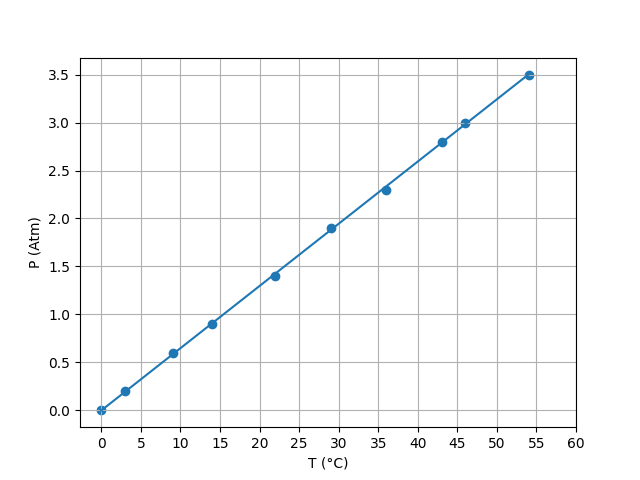
\includegraphics[scale=0.8]{plot-1.png}


\subsection*{Cálculo de variables termodinámicas asociadas a las transformaciones}


Las variables a calcular son:

\begin{itemize}
    \item  $n$: Cantidad de sustancia (mol)
    \item  $W$: Trabajo realizado por el sistema (J)
    \item  $Q$: Calor transferido al sistema (J)
    \item  $\Delta U$: Variación de la energía interna del sistema (J)
    \item  $\Delta H$: Variación de la entalpía del sistema (J)\\
\end{itemize}

\newpage

Para calcular $n$, usamos la ecuación de estado de los gases ideales y la ajustamos al caso particular del sistema.

Primero necesitamos el valor de la pendiente $a$ de la regresión lineal, esto es \fbox{$a = \frac{\Delta P}{\Delta T}$}.\\

Este valor lo obtenemos con el mismo script de python, y para los datos tomados es $0.065\ atm/^\circ{C}$.

Esto en $Pa/K$ es $6570.60$

Podemos calcular el número de moles sabiendo el valor de $a$:

\begin{center}
    $$n = a\cdot \frac{V}{R}$$

    $$n = 6570.60 Pa/K \cdot \frac{0.00073 m^3}{8.31 J/mol\cdot K}$$

    $$n = 0.58\ mol$$
\end{center}


El trabajo realizado por el sistema ($W$) es 0, pues el volumen del gas es constante.


\begin{center}

    $W = 0$

\end{center}



Para calcular el calor transferido al sistema ($Q$), tomamos en cuenta que el gas usado es un gas diatómico, por lo
tanto el calor específico de este es $\frac{5}{2}\cdot R$, siendo $R$ la constante universal de los gases ideales:


\begin{center}
    $$Q = nCv\Delta T$$

    $$Q = (0.58 mol)(\frac{5}{2} \cdot 8.31)(327.2 ^\circ{K})$$

    $$Q = 3.9 kJ$$
\end{center}

Ahora podemos calcular la variación de la energía interna del sistema ($\Delta U$).\\

\begin{center}
    $\Delta U = Q + W$
\end{center}

Entonces:

\begin{center}
    $$\Delta U = 3.9kJ$$
\end{center}

De esto también se deduce que la variación de entalpía ($\Delta H$) = $\Delta U$ = $3.39kJ$


\newpage

Así, tenemos que para estas transformaciones isocóricas:

\begin{itemize}
    \item $n = 0.58 mol$
    \item $W = 0.0$
    \item $Q = 3.9kJ$
    \item $\Delta U = 3.9kJ$
    \item $\Delta U = 3.9kJ$
\end{itemize}

\end{document}